% ---------------------------------------------------------------------
\documentclass{article}

\usepackage{nberpreamble}
\title{\bfseries Notes on Simulating Power}
\author{\sffamily Prepared by Mauricio C\'aceres}
\date{\sffamily \today}

\usepackage{fontspec}
\fontspec{Open Sans}
\setmainfont{Open Sans Light}
% \setmathfont{Cambria Math}

\usepackage{pgfplots}  % awesome plotting
\usepackage{tikz}      % vector graphics!
\usetikzlibrary{
  arrows,
  patterns,
  positioning,
  calc,
  fit,
  intersections,
  decorations.text,
  decorations.markings,
  decorations.pathmorphing,
  shadows.blur
}

\pgfplotsset{
  compat      = newest,
  axis x line = middle,
  axis y line = center,
  tick align  = outside,
  yticklabels = {,,},
  xticklabels = {,,},
  xtick       = {0},
  ytick       = {0}
}

\renewcommand{\displayoptions}{
  % \maketitle
  % \pagenumbering{arabic}
}

% ---------------------------------------------------------------------
\begin{document}
\displayoptions

\begin{figure}[H]
  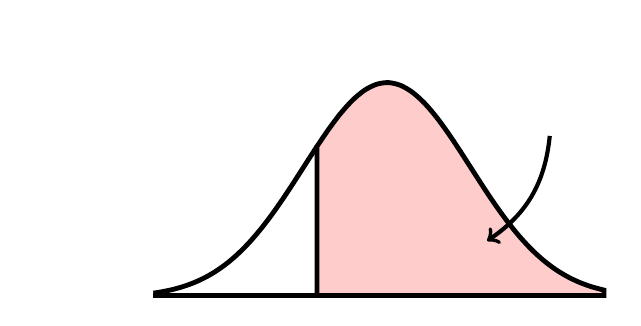
\begin{tikzpicture}
    \begin{axis}[name=plot1
      %,title=
      ,width=9cm
      ,height=5cm
      ,ymin=0
      ,ymax=0.5
      ,xmin=-1.5
      ,xmax=5.5
      ,domain=-6:6
      ,axis line style={white}
      % ,axis line style={ultra thick}
      ]
      \addplot [line width = 1.75pt, fill=red!20,smooth,domain=1.96:5.4] {exp( - (x - 2.8)^2 / 2) / sqrt(2 * pi * 1)} \closedcycle;
      \addplot [line width = 1.75pt, smooth,domain=0:1.96] {exp( - (x - 2.8)^2 / 2) / sqrt(2 * pi * 1)};
      \draw [line width = 3.5pt] (axis cs:0, 0) -- (axis cs:5.4, 0);
      % \draw [line width = 1.5pt, -] (axis cs:2.8, 0) -- (axis cs:2.8, 0.399);
      % \draw [line width = 1.5pt, <->] (axis cs:2, 0.1) -- (axis cs:2.76, 0.1);
      % \node[above] at (axis cs:2.4, 0) {$t_{\kappa}$};
      % \node[above] at (axis cs:2.8, 0.4) {$\widetilde{\beta} / SE$};
      \draw [line width = 1.5pt, ->] (axis cs:4.75, 0.3) to[bend left=25] (axis cs:4, 0.105)
      % node[above] at (axis cs:4.75, 0.3) {$\pi_N(\widetilde{\beta}) = \kappa$};
      ;
    \end{axis}
    % \draw [line width = 1.5pt, dashed] (3.66, 3.33) -- (3.66, 1.5);
  \end{tikzpicture}
  \label{fig:power_of_a_test}
\end{figure}

%----------------------------------------------------------------------
\end{document}
